The Compact C Type Format (CTF) encapsulates all of the information
needed by OpenDTrace to understand C language types such as integers,
strings, floats and structures.  The goal of having another section
just for C type information is to provide a compact representation of
the information that usually appears in the debugging sections of
object files and executables.  CTF only contains data types it
does not contain other debugging infromation, which allows it to be
far more compact.  The debugging sections on a debug build of FreeBSD
in 2017 take up 78 megabytes of space, while the CTF section in the
same kernel tak up only 800 kilobytes. 

\section{On Disk Format}
\label{sec:ctf-on-disk-format}

CTF data is stored in its own ELF section within an object file or
executable.  It is meant to be stored in a format that is both compact
and which is properly aligned so that it can be accessed using the
mmap(2) system call.

\begin{figure}[h]
  \centering
  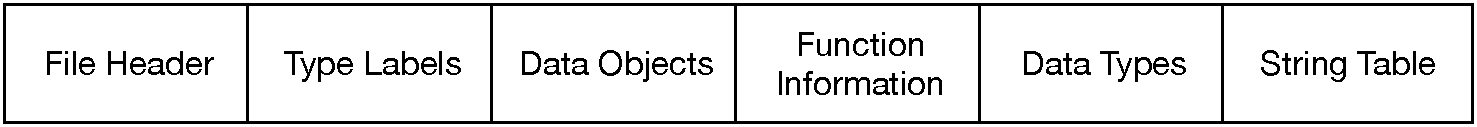
\includegraphics[width=.8\textwidth]{ctf-stable-format}
  \caption{CTF Stable Storage Format}
  \label{fig:ctf-stable-storage-format}
\end{figure}

Figure~\ref{fig:ctf-stable-storage-format} shows all of the components
of the CTF section as they would be found on stable storage.  The file
header stores a magic number and version information, encoding flags,
and the byte offset of each of the sections relative to the end of the
header itself.  If the CTF data has been uniquified against another
set of CTF data, a reference to that data also appears in the the
header.  This reference is the name of the label corresponding to the
types uniquified against.

Following the header is a list of labels, used to group the types
included in the data types section.  Each label is accompanied by a
type ID i.  A given label refers to the group of types whose IDs are
in the range [0, i].

Data object and function records are stored in the same order as they
appear in the corresponding symbol table, except that symbols marked
\verb|SHN_UNDEF| are not stored and symbols that have no type data are padded
out with zeroes.  For each data object, the type ID (a small integer)
is recorded.  For each function, the type ID of the return type and
argument types is recorded.

The data types section is a list of variable size records that
represent each type, in order by their ID.  The types themselves form
a directed graph, where each node may contain one or more outgoing
edges to other type nodes, denoted by their ID.

Strings are recorded as a string table ID (0 or 1) and a byte offset
into the string table.  String table 0 is the internal CTF string
table.  String table 1 is the external string table, which is the
string table associated with the ELF symbol table for this object.
CTF does not record any strings that are already in the symbol table,
and the CTF string table does not contain any duplicated strings.

If the CTF data has been merged with another parent CTF object, some
outgoing edges may refer to type nodes that exist in another CTF
object.  The debugger and libctf library are responsible for
connecting the appropriate objects together so that the full set of
types can be explored and manipulated.


\section{Data Types}
\label{sec:ctf-data-types}

CTF encodes the following ANSI C data types

%%% Local Variables:
%%% mode: latex
%%% TeX-master: "dtrace-specification"
%%% End:
